\documentclass[12pt, a4paper]{article}

\usepackage[margin=1in]{geometry}
\usepackage{amsmath, amssymb, amsthm}
\usepackage{hyperref}
\usepackage{fancyhdr}
\usepackage{graphicx}
\usepackage{tikz}

\theoremstyle{definition}
\newtheorem{definition}{Definition}[section]
\newtheorem{example}{Example}[section]

\theoremstyle{plain}
\newtheorem{theorem}{Theorem}[section]

\newcommand{\Z}{\mathbb{Z}}
\newcommand{\R}{\mathcal{R}}

\setlength{\headheight}{15pt}
\pagestyle{fancy}
\fancyhf{}
\rhead{Post-Quantum Cryptography}
\lhead{NTRU Cryptosystem}
\cfoot{\thepage}

\hypersetup{colorlinks=true, linkcolor=blue, citecolor=magenta}

\begin{document}
\begin{titlepage}
    \centering
    % \vspace*{1.5cm}
    \large A Mid-Semester Report On
    \vspace{0.5cm}

    \LARGE \textbf{Lattice Based Post-Quantum Cryptography}
    
    \vspace{0.5cm}
    
    % \Large \textbf{NTRU Cryptosystem}

    % \vspace{1cm}

    \normalsize By

    \vspace{0.8cm}

    \begin{tabular}{@{} l l l @{}}
        \large \textbf{Shashwat Agrawal}  & \large -- & \large 2024ADPS0197H \\[4pt]
        \large \textbf{Meghraj Goswami} & \large -- & \large 2022A2B41869H \\[4pt]
        \large \textbf{R Revanth Kanna} & \large -- & \large 2022B4AA0926H \\[4pt]
        \large \textbf{Soham Patil} & \large -- & \large 2022B4A30960H \\[4pt]
        \large \textbf{Prashanth Swaminathan} & \large -- & \large ID \\[4pt]
        \large \textbf{Shreya Bhaskar} & \large -- & \large ID \\[4pt]
        \large \textbf{Other Names} & \large -- & \large IDs \\[4pt]
    \end{tabular}
    
    \vspace{1.2cm}

    \large Under the supervision of

    \vspace{0.4cm}

    \large \textbf{Prof.\ Sabyasachi Dey}

    \vspace{1cm}

    \large Submitted in Partial Fulfillment of the Requirements of

    \vspace{0.4cm}

    \large \textbf{MATH F366 / F376}

    \vspace{1.2cm}

    
\includegraphics[width=0.28\textwidth]{bits-logo.png}

    \vspace{1.2cm}

    \large \textbf{BIRLA INSTITUTE OF TECHNOLOGY AND SCIENCE\\
    PILANI (RAJASTHAN)}

    \vspace{0.4cm}

    \large \textbf{HYDERABAD CAMPUS}

    \vspace{0.6cm}

    (March 2026)

\end{titlepage}

\begin{abstract}
Quantum computing is moving at a rapid pace and it is starting to break the classical public-key cryptography we use now. Problems like integer factorization and discrete logarithms, which used to be hard, are becoming easier for quantum computers. That is why Post-Quantum Cryptography (PQC) is garnering a lot of attention. Lattice-based methods are a huge part of PQC because they rely on high level math problems that quantum computers struggle with.\\

This project dives into lattice theory and how to reduce lattice bases. It focuses on the LLL algorithm, created by Arjen Lenstra, Hendrik Lenstra, and László Lovász, and also the more complex BKZ algorithm. The project explains what lattices are mathematically, how Gram-Schmidt orthogonalization works, what size reduction means and the Lovász condition. It encompasses step-by-step algorithm details and examples to make it clearer.\\

We then examine how these reduction methods apply to hard problems such as the Shortest Vector Problem (SVP) and the Closest Vector Problem (CVP), which are central to lattice cryptanalysis. Overall, this project highlights the mathematical foundations and cryptographic importance of lattice reduction in the context of post-quantum security.
\end{abstract}

\newpage

\section*{Acknowledgements}

I would like to extend my sincere gratitude to all those who guided and supported me throughout this project. First, I sincerely thank my project mentor,
Prof.\ Sabyasachi Dey, for his constant guidance, support, and valuable feedback, which were instrumental in the successful completion of this work. I also thank the Department of Mathematics, BITS Pilani Hyderabad Campus, for providing the necessary resources and insights. I extend my heartfelt thanks to my fellow project teammates
for their dedication, teamwork, and collaboration at every stage. Finally, I am profoundly grateful to my family and friends for their encouragement and patience throughout.

\newpage
\tableofcontents
\newpage

\section{Literature Review -- Shreya Bhaskar}

Lattice theory is a significant area in computational mathematics and modern cryptography. To build post-quantum cryptography, we need to solve many hard geometric problems in lattices, such as Shortest Vector Problem (SVP) and Closest Vector Problem (CVP). Interestingly, these problems are considered to be hard even for quantum computers.
The LLL algorithm for lattice basis reduction was introduced by Arjen Lenstra, Hendrik Lenstra and László Lovász in 1982. The first polynomial time algorithm for producing a reduced lattice basis with guaranteed optimality, the LLL algorithm is based on the Gram-Schmidt procedure, the size-reduction algorithm and the Lovász condition to produce a basis with short, almost orthogonal vectors. It has been widely used in number theory, cryptanalysis, integer programming and coding theory. While the LLL algorithm is considered efficient, its reduction strength is moderate, which makes it more applicable to approximating SVP instances.
The Block Korkine-Zolotarev (BKZ) algorithm is a method for achieving stronger reductions from the approximate Shortest Vector Problem (SVP) than the original LLL algorithm. The BKZ algorithm reduces lattice vectors in blocks and attempts to solve the SVP locally in each block. Increasing the block size generally leads to better reduction efficiency, but the running time increases exponentially. The BKZ algorithm has been used in the majority of lattice cryptanalysis results against lattice-based cryptographic schemes, and is a common tool for assessing the security of lattice-based cryptography.
So far, a number of works have demonstrated that lattice basis reduction algorithms can be used for both theoretical and cryptographic purposes. In this work, we examine in greater detail two of the most widely used reduction algorithms in the lattice reduction literature, LLL and BKZ, in order to gain insight into the time complexity reduction trade-offs and the resulting security implications for certain post-quantum cryptographic proposals based on lattices.

\newpage

% --------------------------------------------------------------------

\part{Basics of a Lattice -- R Revanth Kanna and Soham Patil}

\section{Introduction to Lattices}

\subsection{Definition and Basis}
A lattice $L$ in $\mathbb{R}^{n}$ is the set of all integer linear combinations of $m$ linearly independent vectors $B=\{v_{1},v_{2},...,v_{m}\}$ in $\mathbb{R}^{n}$ (and where $m\le n)$. The set $B$ is called a basis of $L$, and we write $L=L(B)$. The dimension of $L$ is $n$, and the rank of $L$ is $m$. We will henceforth assume that the basis vectors $v_{1},v_{2},...,v_{m}$ are in $\mathbb{Z}^{n}$. Thus, $L=\{x_{1}v_{1}+x_{2}v_{2}+\cdot\cdot\cdot+x_{m}v_{m}:x_{1},x_{2},...,x_{m}\in\mathbb{Z}\}\subseteq\mathbb{Z}^{n}$. $L$ is called an integer lattice.

Let $B$ be the $n\times m$ matrix whose columns are the basis vectors $v_{1},...,v_{m}$. Then $L=\{Bx:x\in\mathbb{Z}^{m}\}$.

\subsection{Full-Rank Lattice}
A full-rank lattice $L$ in $\mathbb{R}^{n}$ is a lattice in $\mathbb{R}^{n}$ of rank $n$. Note that a basis $B=\{v_{1},v_{2},...,v_{n}\}$ for a full-rank lattice in $\mathbb{R}^{n}$ is also a basis for the vector space $\mathbb{R}^{n}$. Henceforth, unless otherwise stated, all lattices and sublattices will be full-rank (and integer).

\textbf{Example 1 (Small Lattice):}
Let $n=2$ and $B_{1}=\{(1,0),(0,1)\}$. Then $L_{1}=L(B_{1})=\{B_{1}x:x\in\mathbb{Z}^{2}\}$, where
$$B_{1}=\begin{bmatrix}1&0\\ 0&1\end{bmatrix}$$. Thus, $L_{1}=\mathbb{Z}^{n}$.

\subsection{Fundamental Parallelepiped}
Let $L=L(B)$ be a lattice in $\mathbb{R}^{n}$, where $B=\{v_{1},v_{2},...,v_{n}\}$. The fundamental parallelepiped of $L$ is $P(B)=\{a_{1}v_{1}+a_{2}v_{2}+\cdot\cdot\cdot+a_{n}v_{n}:a_{i}\in[0,1)\}$. Equivalently, $P(B)=\{Bx:x\in[0,1)^{n}\}$. $P(B)$ can be used to partition $\mathbb{R}^{n}$ into non-overlapping regions.

\subsection{Sublattices}
Let $L$ and $L'$ be lattices in $\mathbb{R}^{n}$. Then $L'$ is a sublattice of $L$ if $L^{\prime}\subseteq L$.

\textbf{Example 2 (Sublattice):}
Let $n=2$ and $B_{2}=\{(2,0),(0,1)\}$. Then $L_{2}=L(B_{2})=\{B_{2}x:x\in\mathbb{Z}^{2}\}$, where 
$$B_{2}=\begin{bmatrix}2&0\\ 0&1\end{bmatrix}$$. $L_{2}$ a sublattice of $L_{1}$. $L_{2}\ne L_{1}$ since $(1,0)\in L_{1}$, but $(1,0)=\frac{1}{2}\cdot(2,0)+0\cdot(0,1)\notin L_{2}$.

\subsection{Equivalence of Bases}
$L_{2}=L(\{(2,0),(0,1)\})$ and $L_{3}=L(\{(-2,-2),(4,3)\})$ are the same lattice, but described using different bases. The basis $B_{2}=\{(2,0),(0,1)\}$ is "nicer" than the basis $B_{3}=\{(-2,-2), (4,3)\}$ since the vectors in $B_{2}$ are "shorter" by Euclidean and "orthogonal" to each other.

\begin{theorem}[Characterization of lattice bases]
Let $L=L(B_{1})$ be an $n$-dimensional (integer) lattice. Then an $n\times n$ integer matrix $B_{2}$ is also a basis for $L$ if and only if $B_{1}=B_{2}U$, where $U$ is an $n\times n$ matrix with integer entries and with $\det(U)=\pm1$. Such a matrix $U$ is called unimodular.
\end{theorem}
\begin{proof}
($\Rightarrow$) Suppose that $B_{1}$ and $B_{2}$ are both bases for $L\subseteq\mathbb{R}^{n}$. Since $B_{1}$ is a basis for $L$, and since the vectors in $B_{2}$ are in $L$, we can write $B_{2}=B_{1}U$ for some invertible matrix $U\in\mathbb{Z}^{n\times n}$. Similarly, we can write $B_{1}=B_{2}V$ for some invertible matrix $V\in\mathbb{Z}^{n\times n}$. Now, $B_{1}=B_{2}V=(B_{1}U)V=B_{1}(UV)$. Since $B_{1}$ is invertible, we have $UV=I_{n}$. Thus, $\det(U)\det(V)=1$, and hence $\det(U)=\pm1$ and $\det(V)=\pm1$.

($\Leftarrow$) Conversely, assume $B_{2}=B_{1}U$ for some unimodular matrix $U \in \mathbb{Z}^{n \times n}$ with $\det(U)=\pm1$. Because $U$ has integer entries, any integer linear combination of the columns of $B_2$ is also an integer linear combination of the columns of $B_1$, giving $L(B_{2}) \subseteq L(B_{1})$. Because $\det(U)=\pm1$, its inverse $U^{-1}$ also has integer entries. From $B_{1}=B_{2}U^{-1}$, it symmetrically follows that $L(B_{1}) \subseteq L(B_{2})$. Therefore, $L(B_{1}) = L(B_{2})$.
\end{proof}

\subsection{Volume of a Lattice}
Let $L=L(B)$ be a lattice. The volume of $L$ is $vol(L)=|\det(B)|$. The volume of a lattice is the "volume" of the fundamental parallelepiped of the lattice.

\begin{theorem}[Volume is invariant of basis]
The volume is an invariant of $L$, i.e., it doesn't depend on the basis $B$ chosen for $L$.
\end{theorem}
\begin{proof}
Let $B_{1}$ and $B_{2}$ be two bases for the same lattice $L$. By the characterization of lattice bases, $B_{2}=B_{1}U$ for some unimodular matrix $U$ with $\det(U)=\pm1$. The volume generated by $B_{2}$ is $vol(L(B_{2})) = |\det(B_{2})| = |\det(B_{1}U)|$. Since the determinant of a product is the product of determinants, this equals $|\det(B_{1})\det(U)| = |\det(B_{1})(\pm1)| = |\det(B_{1})| = vol(L(B_{1}))$. Thus, the volume is invariant.
\end{proof}

\begin{theorem}[Volume of a Sublattice]
Suppose that $L_{1}\subseteq L_{2}$. Then $vol(L_{1})\ge vol(L_{2})$.
\end{theorem}
\begin{proof}
Let $B_{1}$ be a basis for $L_{1}$ and $B_{2}$ be a basis for $L_{2}$. Because $L_{1}\subseteq L_{2}$, the basis vectors of $B_{1}$ must belong to $L_{2}$. Therefore, there exists an integer matrix $M$ such that $B_{1}=B_{2}M$. The volume of $L_{1}$ is $vol(L_{1}) = |\det(B_{1})| = |\det(B_{2}M)| = |\det(B_{2})||\det(M)|$. This simplifies to $vol(L_{2})|\det(M)|$. Because $M$ is an integer matrix for full-rank lattices, its determinant is a non-zero integer, meaning $|\det(M)| \ge 1$. Consequently, $vol(L_{1}) \ge vol(L_{2})$.
\end{proof}

\vspace{0.5cm}

\subsection*{1.7 \quad Shortest Vector Problem (SVP)}

\noindent \textbf{Definition 1.2.} \textit{Given a lattice $L$, find a nonzero $v \in L$ minimizing the Euclidean norm $\|v\|_2$.}

\vspace{0.3cm}
The length of the shortest non-zero vector is denoted by the first successive minimum:
\[
\lambda_1(L) = \min_{v \in L\setminus\{0\}} \|v\|_2
\]

Exact SVP is known to be NP-hard under randomized reductions in high dimensions. In cryptography, we typically rely on the Approximate SVP ($\text{SVP}_\gamma$), where the goal is to find a vector $v$ such that $\|v\| \leq \gamma \cdot \lambda_1(L)$ for a given approximation factor $\gamma$.

\vspace{0.5cm}

\subsection*{1.8 \quad Closest Vector Problem (CVP)}

\noindent \textbf{Definition 1.3.} \textit{Given a target vector $t \in \mathbb{R}^n$ that is not necessarily in $L$, find a lattice vector $v \in L$ that minimizes the distance $\|t - v\|_2$.}

\vspace{0.3cm}
Mathematically, this means finding $v \in L$ such that $\|t - v\| \leq \|t - w\|$ for all $w \in L$. CVP models the decoding of noisy messages: if $t = mB + e$ for a small error $e$, finding the closest lattice point recovers $mB$ and removes the error. Like SVP, exact CVP is NP-hard.

\vspace{0.5cm}

\subsection*{1.9 \quad Hermite's Theorem}

\noindent \textbf{Theorem 1.4.} \textit{For an $n$-dimensional lattice $L$, there exists a constant $\gamma_n$ (Hermite's constant) such that:}
\[
\lambda_1(L)^2 \leq \gamma_n (\text{vol}(L))^{2/n}.
\]

\vspace{0.3cm}
This theorem guarantees a universal upper bound on the length of the shortest vector in terms of the lattice's volume. While the exact value of $\gamma_n$ is only known for small dimensions, it scales linearly with $n$, ensuring short vectors mathematically exist even if finding them computationally is difficult.

\vspace{0.5cm}

\subsection*{1.10 \quad Minkowski's Theorem}

\noindent \textbf{Theorem 1.5.} \textit{Let $L$ be a lattice in $\mathbb{R}^n$ and $S$ a symmetric convex body. If}
\[
\text{vol}(S) > 2^n\text{vol}(L)
\]
\textit{then $S$ contains a nonzero lattice point.}

\vspace{0.3cm}
This converts volume information into the existence of lattice points. By applying this theorem to an $n$-dimensional hypersphere, Minkowski established a direct bound on the shortest vector: $\lambda_1(L) \leq \sqrt{n}(\text{vol}(L))^{1/n}$.

\newpage

% --------------------------------------------------------------------

\part{Lattice Basis Reduction -- Prashanth Swaminathan}

\section{Introduction}

A lattice is a discrete subset of $\mathbb{R}^n$ generated by integer linear combinations of linearly independent vectors. If $b_1, b_2, \dots, b_n$ are basis vectors, the lattice generated by them is

\[
L = \{a_1b_1 + a_2b_2 + \dots + a_nb_n \mid a_i \in \mathbb{Z}\}.
\]

A lattice can have infinitely many different bases. Some bases contain long and nearly parallel vectors. Others contain shorter vectors that are closer to orthogonal. Lattice basis reduction algorithms transform an arbitrary basis into a reduced basis containing shorter and more orthogonal vectors.

\subsection{Why do we need Lattice Basis Reduction Methods}

Many computational problems produce lattice bases that are poorly conditioned. Long vectors that are nearly linearly dependent make calculations inefficient and obscure the structure of the lattice.

Basis reduction improves the basis quality by shortening the vectors and reducing their mutual angles. This makes it easier to analyze the geometry of the lattice.

These techniques are widely used in cryptanalysis, integer programming, number theory, and coding theory. In particular, they are important for approximating difficult lattice problems such as the Shortest Vector Problem (SVP) and the Closest Vector Problem (CVP).

%--------------------------------------------------
\section{LLL}

\subsection{History and Development of LLL}

The LLL algorithm was introduced in 1982 by Arjen Lenstra, Hendrik Lenstra, and László Lovász. It was the first polynomial-time algorithm capable of computing a reduced lattice basis with provable guarantees.

The algorithm quickly became a fundamental tool in computational mathematics and cryptography. It has applications in polynomial factorization, solving Diophantine equations, and analyzing cryptographic constructions.

%--------------------------------------------------
\subsection{Mathematical Formulation of LLL}

Let $B=(b_1,b_2,\dots,b_n)$ be a lattice basis in $\mathbb{R}^m$.

Using Gram-Schmidt orthogonalization we compute vectors

\[
b_1^*,b_2^*,\dots,b_n^*
\]

and coefficients

\[
\mu_{i,j}=\frac{\langle b_i,b_j^*\rangle}{\langle b_j^*,b_j^*\rangle}, \quad j<i
\]

The LLL reduction satisfies two conditions.

\textbf{Size Reduction}

\[
|\mu_{i,j}| \le \frac{1}{2}, \quad j<i
\]

\textbf{Lovász Condition}

\[
\delta ||b_{k-1}^*||^2 \le ||b_k^*+\mu_{k,k-1}b_{k-1}^*||^2
\]

where

\[
\frac{1}{4} < \delta < 1
\]

and commonly $\delta = 3/4$.

%--------------------------------------------------
\subsection{Algorithm for Applying LLL}

\begin{enumerate}

\item Compute the Gram-Schmidt orthogonalization of the basis vectors.

\item Perform size reduction

\[
b_i = b_i - \text{round}(\mu_{i,j})b_j
\]

until $|\mu_{i,j}| \le \frac{1}{2}$.

\item Check the Lovász condition.

\item If the condition holds, move to the next vector.

\item If the condition fails, swap $b_k$ and $b_{k-1}$.

\item Recompute Gram-Schmidt coefficients and repeat until the basis is reduced.

\end{enumerate}

%--------------------------------------------------
\subsection{Standard Solved Example}

Consider the lattice basis

\[
b_1=(1,1,1), \quad b_2=(-1,0,2), \quad b_3=(3,5,6)
\]

\textbf{Step 1: Gram-Schmidt Orthogonalization}

\[
b_1^* = b_1 = (1,1,1)
\]

Compute

\[
\mu_{2,1}=\frac{b_2\cdot b_1^*}{b_1^*\cdot b_1^*}
\]

\[
b_2\cdot b_1^* = (-1)(1)+0(1)+2(1)=1
\]

\[
b_1^*\cdot b_1^*=3
\]

\[
\mu_{2,1}=\frac{1}{3}
\]

Thus

\[
b_2^* = b_2-\mu_{2,1}b_1^*
\]

\[
b_2^*=(-1,0,2)-\frac13(1,1,1)
\]

\[
b_2^*=(-\tfrac43,-\tfrac13,\tfrac53)
\]

Next compute

\[
\mu_{3,1}=\frac{b_3\cdot b_1^*}{b_1^*\cdot b_1^*}
\]

\[
b_3\cdot b_1^* = 3+5+6=14
\]

\[
\mu_{3,1}=\frac{14}{3}
\]

Similarly

\[
\mu_{3,2}=\frac{b_3\cdot b_2^*}{b_2^*\cdot b_2^*}
\]

After computing these coefficients, the algorithm performs size reduction and checks the Lovász condition. If the Lovász condition is violated, the vectors are swapped and the process repeats until a reduced basis is obtained.

The resulting reduced basis consists of shorter vectors that are closer to orthogonal than the original basis.

%--------------------------------------------------
\section{BKZ}

\subsection{What is BKZ}

BKZ (Block Korkine-Zolotarev) is an extension of the LLL algorithm that performs reduction on blocks of vectors instead of single vectors.

The algorithm was developed to produce stronger lattice reductions. It is widely used in modern lattice cryptanalysis and security evaluation of lattice-based cryptography.

%--------------------------------------------------
\subsection{Mathematical Formulation of BKZ}

Let $B=(b_1,b_2,\dots,b_n)$ be a lattice basis.

BKZ works with a block size $\beta$.

For each block

\[
(b_i,b_{i+1},\dots,b_{i+\beta-1})
\]

the algorithm attempts to solve the Shortest Vector Problem in the projected lattice defined by that block.

A shorter vector found within the block replaces part of the basis, and the entire basis is LLL-reduced again.

Increasing the block size improves reduction quality but significantly increases computation time.

%--------------------------------------------------
\subsection{Algorithm for Applying BKZ}

\begin{enumerate}

\item Begin with an LLL-reduced basis.

\item Select a block size $\beta$.

\item For each block of $\beta$ vectors, construct the projected lattice.

\item Attempt to solve the Shortest Vector Problem in that block.

\item Insert the resulting short vector into the basis.

\item Apply LLL reduction again.

\item Repeat until no further improvement occurs.

\end{enumerate}

%--------------------------------------------------
\subsection{Comparison with LLL}

The LLL algorithm runs in polynomial time and is computationally efficient. However, the quality of the reduced basis is moderate.

BKZ produces significantly shorter vectors by solving local shortest vector problems within blocks. This produces stronger reductions and is more effective for difficult lattice problems.

The main drawback of BKZ is computational cost. As the block size increases, the algorithm becomes much slower.

In practical cryptanalysis, LLL is often used as a preprocessing step, while BKZ is applied when stronger reductions are required.

%--------------------------------------------------
\subsection*{Illustration of BKZ Block Processing}

\begin{center}
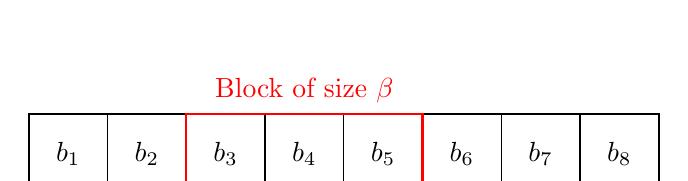
\begin{tikzpicture}[scale=1]

\draw[thick] (0,0) rectangle (8,1);

\foreach \x in {1,2,3,4,5,6,7}
\draw (\x,0) -- (\x,1);

\node at (0.5,0.5) {$b_1$};
\node at (1.5,0.5) {$b_2$};
\node at (2.5,0.5) {$b_3$};
\node at (3.5,0.5) {$b_4$};
\node at (4.5,0.5) {$b_5$};
\node at (5.5,0.5) {$b_6$};
\node at (6.5,0.5) {$b_7$};
\node at (7.5,0.5) {$b_8$};

\draw[red, thick] (2,0) rectangle (5,1);

\node[red] at (3.5,1.3) {Block of size $\beta$};

\end{tikzpicture}
\end{center}

The highlighted region represents the block on which the algorithm performs stronger reduction before sliding the block forward along the basis.

\newpage

% --------------------------------------------------------------------

\part{Applications of LLL to Cryptanalysis -- Shashwat Agrawal}

\section{Overview}

The LLL(Lenstra Lenstra Lovez) is a major tool in cryptography. It has broken older system like the knapsack system. It is also the primary tool for the modern systems such as GGH and NTRU. Further, the LLL can also be used to attack the RSA crypto system under certain defined conditions.

In the following examples lower dimension matrices have been used for illustrative purposes and better explanation. In practical basis higher dimension matrices are used for security purposes.

\section{Congruential Cryptosystems}

In a standard congruential cipher, Alice selects a public modulus $q$ alongside two small secret integers, $f$ and $g$. The public key is broadcast as $h \equiv f^{-1}g \pmod{q}$. Eve's objective is to compute the private key $f$ knowing only $q$ and $h$.

This can be mapped to a lattice problem. Eve constructs a lattice $L$ spanned by the vectors:
\[
    \mathbf{v}_1 = (1, h) \quad \text{and} \quad \mathbf{v}_2 = (0, q)
\]
Because the vector $(f, g)$ is a linear combination of this basis and is constrained to be small, it will likely represent the shortest nonzero vector in $L$.

\subsection{Worked Example: Breaking the Congruential Cipher}

\textbf{Problem Setup:} Let $q = 122430513841$ and $h = 39245579300$. How can an attacker recover the private keys $f$ and $g$?

\textbf{Solution via LLL:}
Eve generates the lattice from the vectors:
\[
    \mathbf{v}_1 = (1,\, 39245579300) \quad \text{and} \quad \mathbf{v}_2 = (0,\, 122430513841)
\]
Applying Gaussian lattice reduction (a 2D analog of LLL) takes exactly 11 iterations. The algorithm outputs a new, reduced basis containing much shorter vectors:
\[
    (-231231,\, -195698) \quad \text{and} \quad (-368222,\, 217835)
\]
The shortest vector in this reduced basis represents the secret variables. Ignoring the irrelevant change of sign, Eve successfully retrieves Alice's private keys:
\[
    f = 231231 \quad \text{and} \quad g = 195698
\]

\section{Knapsack (Subset-Sum) Problems}

The knapsack problem defined by a set of weights $M = (m_1, \dots, m_n)$ and a target sum $S$ can be made easier by turning it into a LLL problem. By assembling a specific basis matrix, the target solution vector is embedded into the lattice $L_{M,S}$. We will be using a very unique matrix to solve the problem. Different types of matrices can be introduced, the main aim is to turn the knapsack problem to a LLL problem.

\subsection{Worked Example: Solving the Knapsack with LLL}

\textbf{Problem Setup:} Consider the knapsack instance with weight vector $M = (89, 243, 212, 150, 245)$ and target sum $S = 546$. Find the specific combination of weights that sums exactly to $S$.

\textbf{Solution via LLL:}
We construct a basis matrix $A_{M,S}$ where the weights and target are aligned to form the lattice constraints:
\[
    A_{M,S} = 
    \begin{pmatrix}
    2 & 0 & 0 & 0 & 0 & 89 \\
    0 & 2 & 0 & 0 & 0 & 243 \\
    0 & 0 & 2 & 0 & 0 & 212 \\
    0 & 0 & 0 & 2 & 0 & 150 \\
    0 & 0 & 0 & 0 & 2 & 245 \\
    1 & 1 & 1 & 1 & 1 & 546
    \end{pmatrix}
\]
Applying the LLL algorithm to the rows of this matrix takes 21 swaps and outputs the following reduced basis matrix:
\[
    \begin{pmatrix}
    -1 & 1 & -1 & 1 & -1 & 0 \\
    1 & -1 & -1 & 1 & -1 & -1 \\
    -1 & -1 & -1 & 1 & 1 & 2 \\
    1 & -1 & -1 & -1 & -1 & 2 \\
    -2 & -2 & 4 & 0 & -2 & 0 \\
    -6 & -4 & -6 & -6 & 0 & -3
    \end{pmatrix}
\]
The shortest vector in the reduced basis (the top row) is $\mathbf{v} = (-1, 1, -1, 1, -1, 0)$. 

To find the subset-sum solution, we write $\mathbf{v}$ as a linear combination of the original basis vectors (the rows of $A_{M,S}$). This linear combination vector is $(-1, 0, -1, 0, -1, 1)$. This translates directly to the correct subset sum:
\[
    -89 - 212 - 245 + 546 = 0
\]
Thus, the items weighing 89, 212, and 245 are the ones that perfectly fill the knapsack.

\textbf{Remark:} When using LLL to solve subset-sum problems, it is helpful to multiply $m_1, \dots, m_n$ and the target $S$ by a large constant $C$. This scales up the expected length of non-target shortest vectors by $C^{1/(n+1)}$, while the target vector's length remains $\sqrt{n}$. The larger distance between the target vector and the rest of the lattice makes it significantly easier for LLL to isolate the correct solution.

\section{GGH Cryptosystem}

This is the most basic cryptosystem to understand what exactly it means, to convert a bad basis to a good basis. In earlier sections, we had to convert the problem first to an  LLL problem, then solve it. Now the problem is already given in the matrix form and is ready to solve.

\subsection{Worked Example: Breaking GGH with Babai's Algorithm}

\textbf{Problem Setup:} Alice's public lattice $L$ is generated by the rows of the following matrix (representing a bad basis):
\[
    \begin{pmatrix}
    -4179163 & -1882253 & 583183 \\
    -3184353 & -1434201 & 444361 \\
    -5277320 & -2376852 & 736426
    \end{pmatrix}
\]
Bob's encrypted message is the vector $\mathbf{e} = (-79081427,\, -35617462,\, 11035473)$. How can Eve find the plaintext message?

\textbf{Solution via LLL:}
Eve cannot effectively use Babai's algorithm on the bad public basis. First, she applies LLL to the lattice $L$ to find a quasi-orthogonal "good" basis:
\[
    \begin{pmatrix}
    36 & -30 & -86 \\
    61 & 11 & 67 \\
    -10 & 102 & -40
    \end{pmatrix}
\]
This new basis has a Hadamard ratio of $H = 0.956083$, meaning it is highly orthogonal. Next, Eve applies Babai's algorithm to find a lattice vector $\mathbf{v}$ that is extremely close to the intercepted ciphertext $\mathbf{e}$. Babai's algorithm returns:
\[
    \mathbf{v} = (79081423,\, 35617459,\, -11035471)
\]
Finally, she writes $\mathbf{v}$ in terms of the original good basis vectors, which immediately retrieves Bob's plaintext:
\[
    \mathbf{m} = (-86,\, 35,\, 32)
\]

\section{Conclusion}

The LLL algorithm was a major breakthrough in the world of cryptography. As seen in the exmaples it can easily break the knapsack, GGH and congruential cryptosystems. Even though it might be ineffective if the dimension sizes of the matrix are increased. But increasing the dimensions after a limit may make the system itself inefficient. Future cryptosystems are made keeping in mind there security against the LLL system.

\newpage

% --------------------------------------------------------------------

\part{NTRU Cryptosystem -- Meghraj Goswami}

\section{Introduction}

The rapid advancement of quantum computing poses a threat to modern cryptographic infrastructure. Shor's algorithm demonstrates that a quantum computer can factor large integers and compute discrete logarithms in polynomial time---$O((\log n)^3)$---completely breaking RSA and Elliptic Curve Cryptography (ECC) at any practical key size in a short time frame~\cite{shor94}.\\

In response, the cryptographic community has shifted towards \textbf{Post-Quantum Cryptography (PQC)}, algorithms that remain secure even against quantum adversaries. The \textbf{NTRU} cryptosystem ($N$-th degree Truncated polynomial Ring Unit), introduced by Hoffstein, Pipher, and Silverman in 1996~\cite{ntru96}, is one of the oldest and most analysed PQC proposals. Its security rests on the hardness of the Shortest Vector Problem (SVP) in certain lattices, for which no efficient quantum algorithm is known as of yet.

Key advantages of NTRU over RSA and ECC\:
\begin{itemize}
    \item No known quantum speedup for the underlying lattice problem.
    \item Fast polynomial operations.
    \item Compact keys: public keys are approximately 700 bytes at the 128-bit security level, versus several kilobytes for RSA at equivalent security.
    \item NTRU has been a prominent fixture in the NIST PQC standardization process.\cite{nistpqc}
\end{itemize}

\section{Mathematical Prerequisites}

\subsection{Groups}

\begin{definition}[Group]
    A \textbf{group} is a pair $(G, \cdot)$ where $G$ is a set and
    $\cdot : G \times G \to G$ is a binary operation satisfying:
    \begin{enumerate}
        \item \textbf{Closure:} $a \cdot b \in G$ for all $a, b \in G$.
        \item \textbf{Associativity:} $(a \cdot b) \cdot c = a \cdot (b \cdot c)$.
        \item \textbf{Identity:} $\exists\, e \in G$ such that $a \cdot e = e \cdot a = a$.
        \item \textbf{Inverses:} For each $a \in G$, $\exists\, a^{-1} \in G$
              with $a \cdot a^{-1} = e$.
    \end{enumerate}
    If additionally $a \cdot b = b \cdot a$ for all $a, b \in G$, the group is
    called \textbf{abelian}.
\end{definition}

\begin{example}[Clock arithmetic $(\Z/12\Z,\, +)$]
    Integers modulo 12 under addition: $10 + 4 \equiv 2 \pmod{12}$.\\
    The identity is $0$; the inverse of $3$ is $9$ since $3 + 9 \equiv 0$.
    This is an abelian group.
\end{example}

\subsection{Rings and Fields}

\begin{definition}[Ring]
    A \textbf{ring} is a triplet $(R, +, \cdot)$ where $(R, +)$ is an abelian group, multiplication is associative, and multiplication distributes over addition. A ring is \textbf{commutative} if $ab = ba$ for all $a, b \in R$.\\
    
    A \textbf{field} is a commutative ring where every nonzero element has a multiplicative inverse.
\end{definition}

\begin{example}
    $\Z$, $\Z/n\Z$, $\mathbb{Q}$, and $\mathbb{R}$ are rings. $\mathbb{Q}$ and $\mathbb{R}$ are fields; $\Z$ is not (the element $2$ has no multiplicative inverse in $\Z$).
\end{example}

\subsection{Polynomial Rings}

\begin{definition}[Polynomial Ring]
    Let $R$ be a commutative ring. The polynomial ring $R[x]$ consists of all formal sums $a_0 + a_1 x + \cdots + a_n x^n$ where $a_i \in R$, under coefficient-wise addition and standard polynomial multiplication.
\end{definition}

\subsection{Convolution Polynomial Rings}

NTRU operates in quotient rings of the following form. Fix a positive integer $N$ and define:
\[
    \R = \frac{\Z[x]}{(x^N - 1)}, \qquad
    \R_q = \frac{(\Z/q\Z)[x]}{(x^N - 1)}, \qquad
    \R_p = \frac{(\Z/p\Z)[x]}{(x^N - 1)}.
\]
The ideal $(x^N - 1)$ enforces $x^N = 1$, so all exponents reduce modulo $N$, and every element can be represented as a polynomial of degree at most $N-1$. Meanwhile, the coefficients are taken modulo $q$ or $p$ in $\R_q$ and $\R_p$ respectively.\\

Multiplication in these rings is the \textbf{convolution product} $\star$:
\[
    c(x) = a(x) \star b(x), \quad c_k = \sum_{\substack{i+j \equiv k \\ \pmod{N}}} a_i b_j.
\]
The wrap-around of higher-degree terms is what gives this product a `cyclic' character.

\begin{example}[Convolution product with $N = 5$]
    Let $a(x) = 1 - 2x + 4x^3 - x^4$ and $b(x) = 3 + 4x - 2x^2 + 5x^3 + 2x^4$.
    Computing coefficient by coefficient using $x^5 = 1$:
    \[
        a(x) \star b(x) = -13 + 20x - 7x^2 + 19x^3 + 5x^4.
    \]
\end{example}

\subsection{Ternary Polynomials}

\begin{definition}[Ternary polynomial set]
    For non-negative integers $d_1, d_2$ with $d_1 + d_2 \le N$,
    \[
        T(d_1, d_2) = \bigl\{ a(x) \in \R \mid
            \text{exactly } d_1 \text{ coefficients equal } +1,\;
            d_2 \text{ equal } -1,\; \text{rest } 0 \bigr\}.
    \]
\end{definition}

These sparse polynomials have small coefficients. Private keys are chosen from $T(d_1, d_2)$ precisely because small coefficients make decryption work (see Section~\ref{sec:correctness}) and make exhaustive search difficult (see Section~\ref{sec:security}).

\subsection{Polynomial Inversion}

Key generation requires computing $f(x)^{-1}$ modulo both $q$ and $p$.
A polynomial $F_q(x)$ is an inverse of $f(x)$ in $\R_q$ if
\[
    f(x) \star F_q(x) \equiv 1 \pmod{q, \, x^N - 1}.
\]
When $N$ and $q$ are both prime, the inverse exists if and only if
$\gcd(f(x),\, x^N - 1) = 1$ in $(\Z/q\Z)[x]$, and can be computed using the
\textbf{extended Euclidean algorithm} for polynomials. If $f$ has no inverse,
a new $f$ is chosen.

\section{Cryptosystem}

\subsection{Public Parameters}

The system is set up with public parameters $(N, p, q, d)$ satisfying:
\begin{itemize}
    \item $N$ is prime.
    \item $\gcd(p, q) = 1$ and $\gcd(N, q) = 1$.
    \item $q > (6d+1)p$ \quad (required for correct decryption; see
          Theorem~\ref{thm:correctness}).
\end{itemize}

\subsection{Key Generation}

Alice generates her keys as follows:
\begin{enumerate}
    \item Choose random private polynomials $f(x) \in T(d+1, d)$ and
          $g(x) \in T(d, d)$.
    \item Compute inverses of $f$ in both quotient rings:
          \[
              F_q(x) = f(x)^{-1} \text{ in } \R_q, \qquad
              F_p(x) = f(x)^{-1} \text{ in } \R_p.
          \]
    \item Compute the \textbf{public key}:
          \[
              h(x) \equiv F_q(x) \star g(x) \pmod{q}.
          \]
\end{enumerate}
\textbf{Private key:} $(f,\, F_p)$. \quad \textbf{Public key:} $h$.

\subsection{Encryption}

Bob represents his plaintext as $m(x) \in \R$ with coefficients in
$\bigl[-\dfrac{p}{2},\, \dfrac{p}{2}\bigr]$.
\begin{enumerate}
    \item Choose a fresh random ephemeral polynomial $r(x) \in T(d, d)$.
    \item Compute the \textbf{ciphertext}:
          \[
              e(x) \equiv p \cdot r(x) \star h(x) + m(x) \pmod{q}.
          \]
\end{enumerate}

Because $r(x)$ is drawn fresh for each encryption, NTRU is a \textit{probabilistic} scheme: encrypting the same message twice yields completely different ciphertexts.

\subsection{Decryption}

Alice recovers $m(x)$ from $e(x)$ in three steps:
\begin{enumerate}
    \item Compute $a(x) \equiv f(x) \star e(x) \pmod{q}$.
    \item \textbf{Center-lift:} adjust each coefficient of $a(x)$ to its
          representative in $\bigl(-q/2,\, q/2\bigr]$.
    \item Recover plaintext: $m(x) \equiv F_p(x) \star a(x) \pmod{p}$.
\end{enumerate}

\subsection{Correctness}\label{sec:correctness}

\begin{theorem}[Decryption correctness]\label{thm:correctness}
    If $q > (6d+1)p$, the decryption procedure recovers $m(x)$ exactly.
\end{theorem}

\begin{proof}
Expanding $a(x)$ and substituting $h(x) = F_q(x) \star g(x)$:
\begin{align*}
    a(x) &\equiv f(x) \star e(x) \pmod{q} \\
         &\equiv f(x) \star \bigl(p \cdot r(x) \star h(x) + m(x)\bigr) \pmod{q} \\
         &\equiv p \cdot f(x) \star F_q(x) \star g(x) \star r(x)
              + f(x) \star m(x) \pmod{q} \\
         &\equiv p \cdot g(x) \star r(x) + f(x) \star m(x) \pmod{q},
\end{align*}
where the last step uses $f \star F_q \equiv 1 \pmod{q}$.\\

The coefficients of $A(x) := p \cdot g \star r + f \star m$ in
$\R$ (before reduction mod $q$) are now bounded. Since $g \in T(d,d)$ and $r \in T(d,d)$,
each coefficient of $g \star r$ is at most $2d$ in absolute value. Since
$f \in T(d+1,d)$ and the coefficients of $m$ are in
$\bigl[-\dfrac{p}{2},\, \dfrac{p}{2}\bigr]$, each coefficient of
$f \star m$ is at most $(2d+1)\dfrac{p}{2}$ in absolute value. Therefore:
\[
    |A_k| \le p \cdot 2d + (2d+1)\dfrac{p}{2} < (6d+1)\dfrac{p}{2} < \dfrac{q}{2}.
\]
Since every coefficient of $A(x)$ already lies in $(-q/2, q/2]$, the
center-lift recovers $A(x)$ \textit{exactly} in $\R$ with no modular wrap-around:
\[
    a(x) = p \cdot g(x) \star r(x) + f(x) \star m(x).
\]
Reducing modulo $p$ kills the blinding term ($p \cdot g \star r \equiv 0 \pmod{p}$):
\[
    F_p \star a \equiv F_p \star f \star m \equiv m \pmod{p}. \qedhere
\]
\end{proof}

\section{Worked Example}

The full protocol is illustrated with the toy parameters $(N, p, q, d) = (7, 3, 41, 2)$.

\subsection{Key Generation}

Alice chooses:
\[
    f(x) = -1 + x^2 + x^3 - x^4 + x^6 \in T(3,2), \quad
    g(x) = -x - x^2 + x^4 + x^6 \in T(2,2).
\]

Using the extended Euclidean algorithm she computes:
\begin{align*}
    F_p(x) &= f(x)^{-1} \pmod{3,\, x^7-1}
            = 1 + x + x^2 + x^3 + 2x^5 + x^6, \\
    F_q(x) &= f(x)^{-1} \pmod{41,\, x^7-1}
            = 37 + 2x + 40x^2 + 21x^3 + 31x^4 + 26x^5 + 8x^6.
\end{align*}

The public key is:
\[
    h(x) = F_q(x) \star g(x) \pmod{41}
         = 30 + 26x + 8x^2 + 38x^3 + 2x^4 + 40x^5 + 20x^6.
\]

\subsection{Encryption}

Bob's plaintext and ephemeral key:
\[
    m(x) = -x^5 + x^3 + x^2 - x + 1, \qquad r(x) = x^6 - x^5 + x - 1.
\]

He computes the ciphertext $e(x) \equiv 3 \cdot r(x) \star h(x) + m(x) \pmod{41}$:
\[
    e(x) = 25 + 3x + 40x^2 + 2x^3 + 4x^4 + 19x^5 + 31x^6.
\]

\subsection{Decryption}

\textbf{Step 1.} Multiply by $f(x)$ mod $41$:
\[
    f(x) \star e(x) \equiv 40 + x + 40x^2 + 40x^3 + 33x^4 + 10x^5 + x^6 \pmod{41}.
\]

\textbf{Step 2.} Center-lift to $(-20.5,\, 20.5]$ (e.g.\ $40 \mapsto -1$,
$33 \mapsto -8$):
\[
    a(x) = -1 + x - x^2 - x^3 - 8x^4 + 10x^5 + x^6.
\]

\textbf{Step 3.} Multiply by $F_p(x)$ mod $3$:
\[
    F_p(x) \star a(x) \pmod{3} = -x^5 + x^3 + x^2 - x + 1 = m(x). \quad \checkmark
\]

\section{Security Analysis}\label{sec:security}

\subsection{Key Recovery Problem}

\begin{definition}[NTRU Key Recovery Problem]
    Given the public key $h(x) \in \R_q$, find ternary polynomials $f(x)$ and
    $g(x)$ such that $f(x) \star h(x) \equiv g(x) \pmod{q}$.
\end{definition}

Since $h = F_q \star g$, knowing $f$ immediately yields $g = f \star h \pmod q$
(and vice versa). The difficulty of this problem is equivalent to finding a
short vector in the \textbf{NTRU lattice}.

\subsection{Brute Force and Meet-in-the-Middle}

An attacker could exhaustively search over all $f \in T(d_1, d_2)$. The search
space has size:
\[
    \binom{N}{d_1}\binom{N-1}{d_2} = \dfrac{N!}{d_1!\, d_2!\, (N-d_1-d_2)!}.
\]
Note that any of the $N$ cyclic rotations of a valid $f$ also decrypts
correctly, so the effective search space is $\#T(d_1,d_2) / N$.

\begin{example}[$(N, p, q, d) = (251, 3, 257, 83)$]
    The search space for $f \in T(84, 83)$ is $\approx 2^{389}$
    polynomials; accounting for $N = 251$ rotations gives roughly $2^{381.6}$
    effective trials. A meet-in-the-middle (birthday) attack takes the square
    root, requiring $\approx 2^{190.8}$ operations---still completely infeasible.
\end{example}

\section{NTRU as a Lattice Cryptosystem (Contribution by R Revanth Kanna)}

While NTRU is defined using polynomial rings, its underlying security relies heavily on lattice problems. Specifically, key recovery can be modeled as a Shortest Vector Problem (SVP), and plaintext recovery can be modeled as a Closest Vector Problem (CVP).

\subsection{The NTRU Lattice}
Let $\mathbf{h}(x)$ be an NTRU public key. The \textbf{NTRU lattice} $L_{\mathbf{h}}^{\text{NTRU}}$ associated with $\mathbf{h}(x)$ is a $2N$-dimensional lattice spanned by the rows of the $2N \times 2N$ matrix $M_{\mathbf{h}}^{\text{NTRU}}$. It is convenient to express this matrix in block form:
\[
M_{\mathbf{h}}^{\text{NTRU}} = \begin{pmatrix} I & \mathbf{h} \\ 0 & qI \end{pmatrix}
\]
where $I$ is the $N \times N$ identity matrix, $0$ is the $N \times N$ zero matrix, and $\mathbf{h}$ represents the circulant matrix formed by the cyclical permutations of the coefficients of $\mathbf{h}(x)$.

\subsection{Key Recovery as a Shortest Vector Problem (SVP)}
The private key in NTRU consists of two "small" polynomials $\mathbf{f}(x)$ and $\mathbf{g}(x)$ such that $\mathbf{f} \star \mathbf{h} \equiv \mathbf{g} \pmod q$. This congruence implies there exists some polynomial $\mathbf{u}(x)$ such that:
\[
\mathbf{f} \star \mathbf{h} = \mathbf{g} + q\mathbf{u}
\]

If we consider the vector $(\mathbf{f}, -\mathbf{u})$ and multiply it by the NTRU basis matrix, we get:
\[
(\mathbf{f}, -\mathbf{u}) \begin{pmatrix} I & \mathbf{h} \\ 0 & qI \end{pmatrix} = (\mathbf{f}, \mathbf{f} \star \mathbf{h} - q\mathbf{u}) = (\mathbf{f}, \mathbf{g})
\]
This proves that the vector $(\mathbf{f}, \mathbf{g})$ is a point in the lattice $L_{\mathbf{h}}^{\text{NTRU}}$. Because $\mathbf{f}$ and $\mathbf{g}$ are chosen to have very small coefficients (mostly $-1, 0, 1$), the vector $(\mathbf{f}, \mathbf{g})$ is unusually short compared to the predictions of the Gaussian heuristic for this lattice. Thus, finding the private key is equivalent to solving the SVP in $L_{\mathbf{h}}^{\text{NTRU}}$.

\subsection{Message Recovery as a Closest Vector Problem (CVP)}
Message recovery in NTRU can similarly be formulated as a CVP. Let $\mathbf{e} \equiv p\mathbf{r} \star \mathbf{h} + \mathbf{m} \pmod q$ be a ciphertext. 

\textbf{Claim 1:} The vector $(p\mathbf{r}, \mathbf{e} - \mathbf{m})$ is in $L_{\mathbf{h}}^{\text{NTRU}}$.
\begin{proof}
From the encryption equation, there exists a polynomial $\mathbf{u}$ such that $p\mathbf{r} \star \mathbf{h} + \mathbf{m} = \mathbf{e} + q\mathbf{u}$, which rearranges to $p\mathbf{r} \star \mathbf{h} - q\mathbf{u} = \mathbf{e} - \mathbf{m}$. 
By multiplying the vector $(p\mathbf{r}, -\mathbf{u})$ by the NTRU matrix:
\[
(p\mathbf{r}, -\mathbf{u}) \begin{pmatrix} I & \mathbf{h} \\ 0 & qI \end{pmatrix} = (p\mathbf{r}, p\mathbf{r} \star \mathbf{h} - q\mathbf{u}) = (p\mathbf{r}, \mathbf{e} - \mathbf{m})
\]
Since it is a linear combination of the rows of the basis matrix, it is in the lattice.
\end{proof}

\textbf{Claim 2:} $(p\mathbf{r}, \mathbf{e} - \mathbf{m})$ is almost certainly the closest lattice vector to the known vector $(0, \mathbf{e})$.
\begin{proof}
The distance between our target $\mathbf{t} = (0, \mathbf{e})$ and the lattice vector $\mathbf{v} = (p\mathbf{r}, \mathbf{e} - \mathbf{m})$ is:
\[
||\mathbf{v} - \mathbf{t}|| = ||(p\mathbf{r}, -\mathbf{m})||
\]
Assuming standard parameters where $\mathbf{r}$ and $\mathbf{m}$ have approximately $d \approx N/3$ non-zero coefficients, the length of this vector is roughly $\sqrt{\frac{2}{3}N(p^2 + 1)}$.
Conversely, the Gaussian heuristic predicts the shortest distance between random points in this lattice to be $\approx 0.484N$. Because the distance to $(p\mathbf{r}, \mathbf{e}-\mathbf{m})$ scales with $\sqrt{N}$ rather than $N$, it is significantly closer than any random lattice point. Hence, solving CVP yields $\mathbf{m}$.
\end{proof}

\textbf{Optimizing the CVP:} We can reduce the lattice-to-target distance without affecting the determinant by using a modified NTRU lattice:
\[
M_{\text{mod}} = \begin{pmatrix} I & p\mathbf{h} \\ 0 & qI \end{pmatrix}
\]
For this modified lattice, using the target $(0, \mathbf{e})$, the closest lattice vector becomes $(\mathbf{r}, \mathbf{e} - \mathbf{m})$. The distance is now $||(\mathbf{r}, -\mathbf{m})|| = \sqrt{||\mathbf{r}||^2 + ||\mathbf{m}||^2}$. This removes the $p^2$ factor from the distance, making the vector even shorter relative to the lattice density, thereby making the CVP significantly easier for lattice reduction algorithms to solve.

\section{Conclusion}

NTRU is a mature, well-studied post-quantum cryptosystem. Its algebraic
foundation in truncated polynomial rings provides a clean mathematical
structure, and its reliance on lattice hardness gives resilience against both
classical and quantum adversaries. Its combination of small key sizes, fast
operations, and strong security evidence makes it one of the most practical
post-quantum proposals available today.

\section{Future Scope of Work}

This project mostly looks at the theory behind LLL and BKZ algorithms and how they work. Several directions remain open for future investigation.

\begin{enumerate}
    \item \textbf{Stronger reduction methods.} Exploring larger block sizes and
          improved heuristics for BKZ could yield faster approximate SVP solvers
          and better practical reduction efficiency.

    \item \textbf{Implementation and experimentation.} Optimized software
          implementations of LLL and BKZ, benchmarked on higher-dimensional
          lattices, would provide concrete data on real-world performance.

    \item \textbf{Impact on cryptographic security parameters.} A deeper study of
          how reduction quality affects the security levels of structured lattices
          used in current PQC schemes is particularly relevant.

    \item \textbf{Alignment with NIST PQC standards.} Extending this work to the
          lattice-based schemes recently standardized by NIST would make the
          analysis directly applicable to real-world deployments.

    \item \textbf{Quantum resistance.} Investigating how well lattice problems
          withstand quantum attacks, and deriving tighter security proofs for
          practical cryptographic constructions, remains an important open problem.
\end{enumerate}

Pushing this work beyond theory into implementation, cryptanalysis, and standardized
PQC schemes would contribute meaningfully to the broader goal of securing
communication in the post-quantum era.

\begin{thebibliography}{9}

    \bibitem{shor94}
    P.W.~Shor. 
    \textit{Algorithms for Quantum Computation: Discrete Logarithms and Factoring}. 
    In: \textit{Proceedings of the 35th Annual IEEE Symposium on Foundations of Computer Science (FOCS)}, 1994, pp. 124--134. 
    \url{https://doi.org/10.1109/SFCS.1994.365700}

    \bibitem{ntru96}
    J.~Hoffstein, J.~Pipher, and J.H.~Silverman. 
    \textit{NTRU\: A Ring-Based Public Key Cryptosystem}. 
    In: \textit{Algorithmic Number Theory (ANTS-III)}, LNCS 1423, Springer, 1998, pp. 267--288. 
    \url{https://doi.org/10.1007/BFb0054868}

    \bibitem{nistpqc}
    \textit{NIST Post-Quantum Standardization Effort}.
    \url{https://csrc.nist.gov/projects/post-quantum-cryptography}

    \bibitem{menezes}
    A.~Menezes.
    \textit{Lattice-Based Cryptography}.
    \url{https://cryptography101.ca/lattice-based-cryptography/}

\end{thebibliography}

\end{document}